\documentclass{article}

% Language setting
% Replace `english' with e.g. `spanish' to change the document language
\usepackage[english]{babel}

% Set page size and margins
% Replace `letterpaper' with `a4paper' for UK/EU standard size
\usepackage[letterpaper,top=2cm,bottom=2cm,left=3cm,right=3cm,marginparwidth=1.75cm]{geometry}

% Useful packages
\usepackage{amsmath}
\usepackage{graphicx}
\usepackage[colorlinks=true, allcolors=blue]{hyperref}

\title{TDT4171 — Artificial Intelligence Methods \\ Assignment 2 - Bayesian networks}
\author{Erik Storås Sommer - 535006}
\date{January 2023}

\begin{document}
\maketitle

Solving the monty hall problem using the graphical network interface GeNIe tool by creating a Bayesian network that represents the problem.

Created three nodes with the following states (door1, door2, door3) and probabilities:

MyChoice:

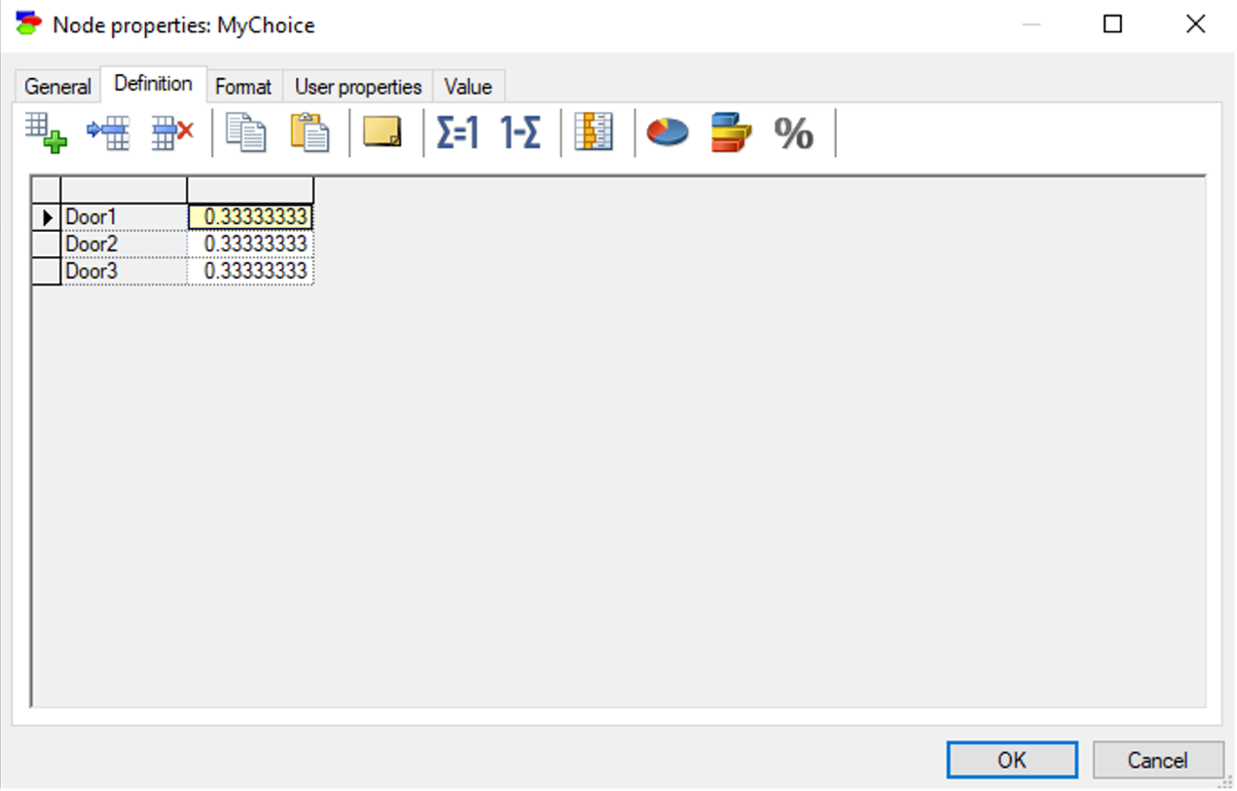
\includegraphics[width=\linewidth]{mychoice.png}

ContainsPrize:

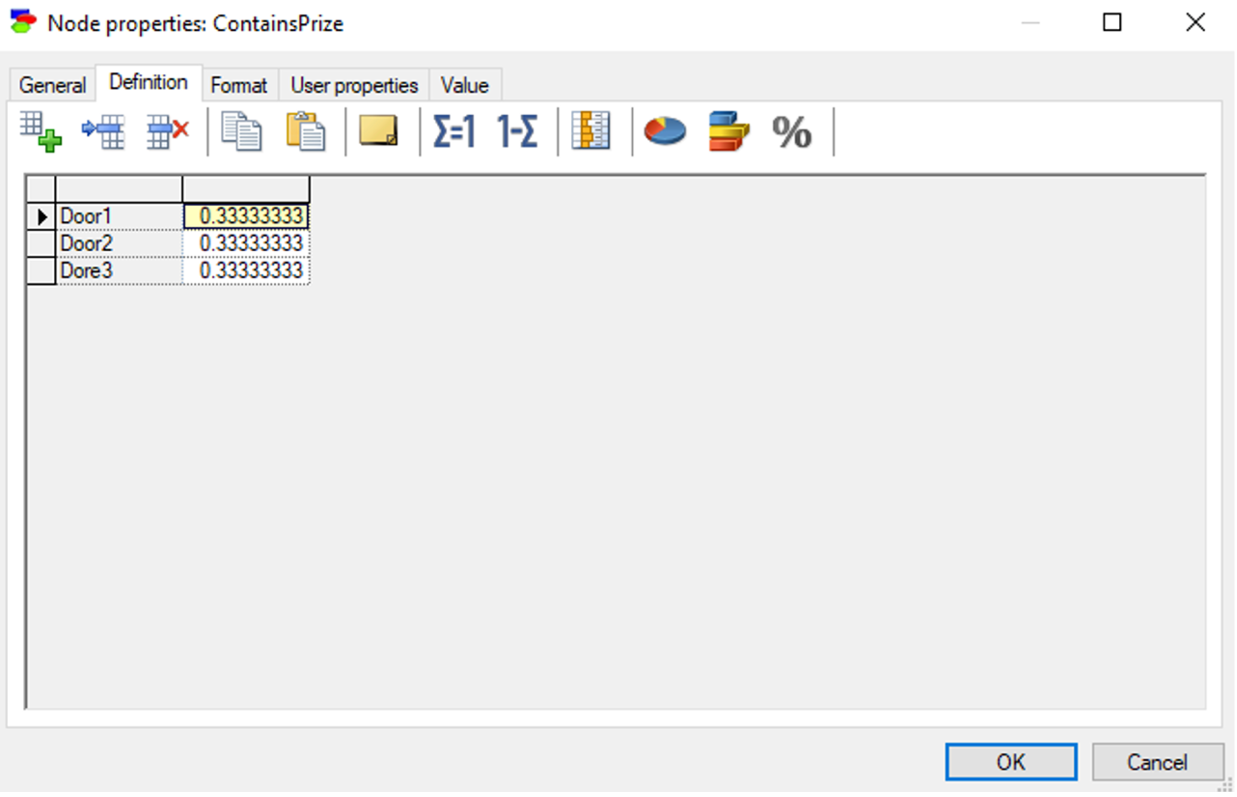
\includegraphics[width=\linewidth]{containsprize.png}

OpenedByOfficial:

\begin{itemize}
    \item The two rules provided gives the following conditional probability table
\end{itemize}


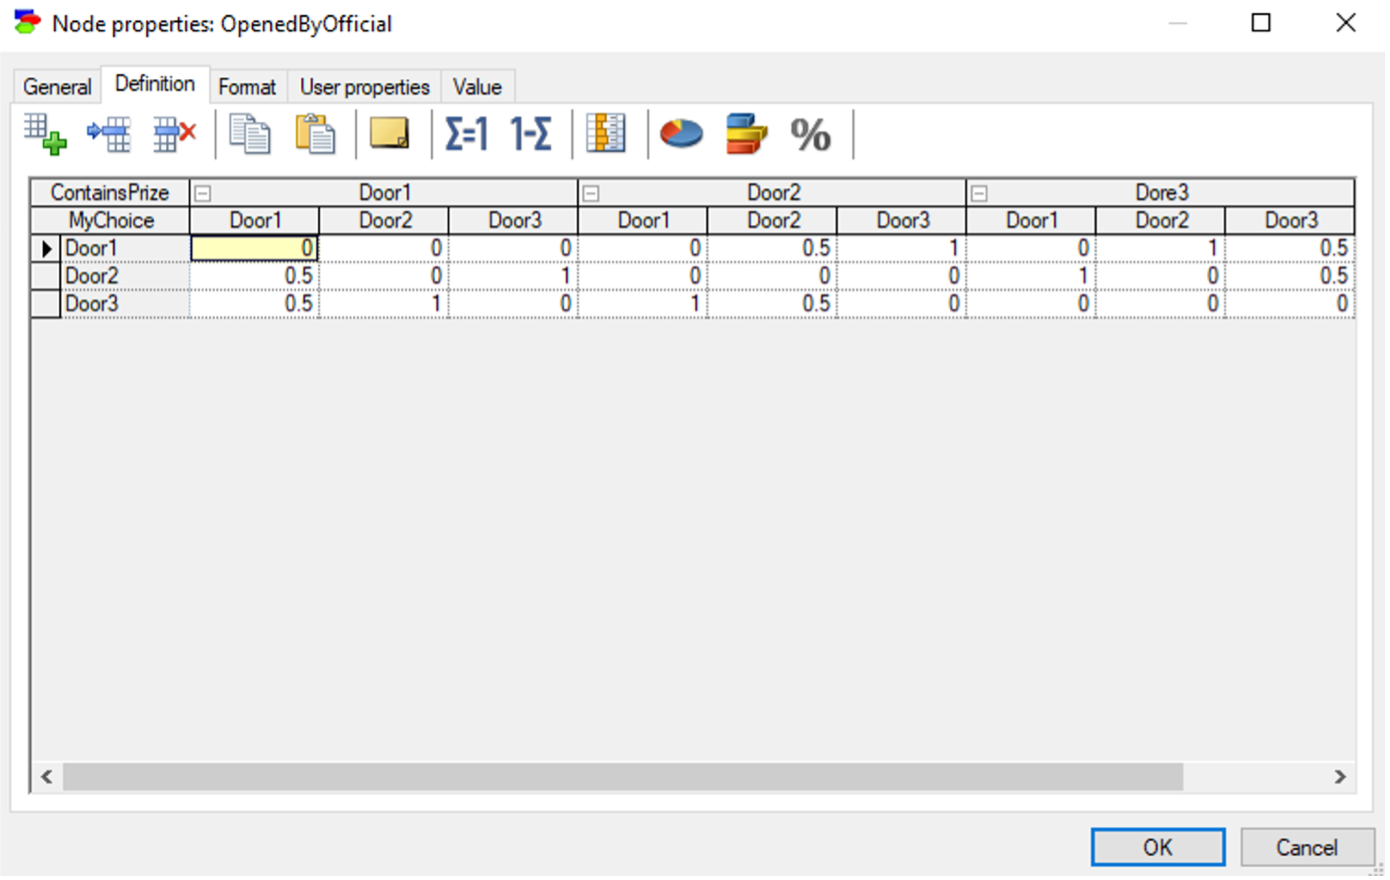
\includegraphics[width=\linewidth]{openedbyofficial.png}


Playing three rounds of the game to see different outcomes:

Play 1:

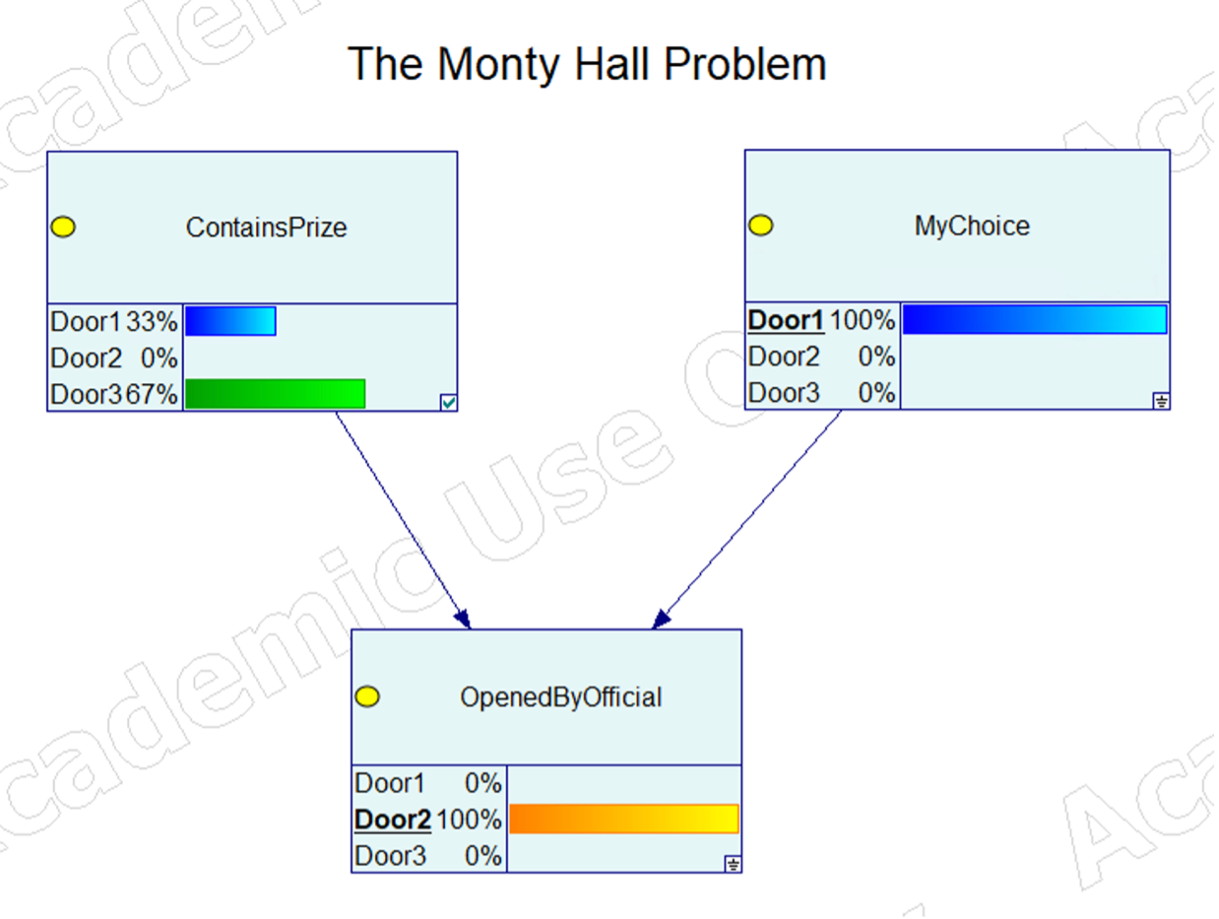
\includegraphics[width=\linewidth]{play1.png}


Result: Highest probability to win if switching door

Play 2:

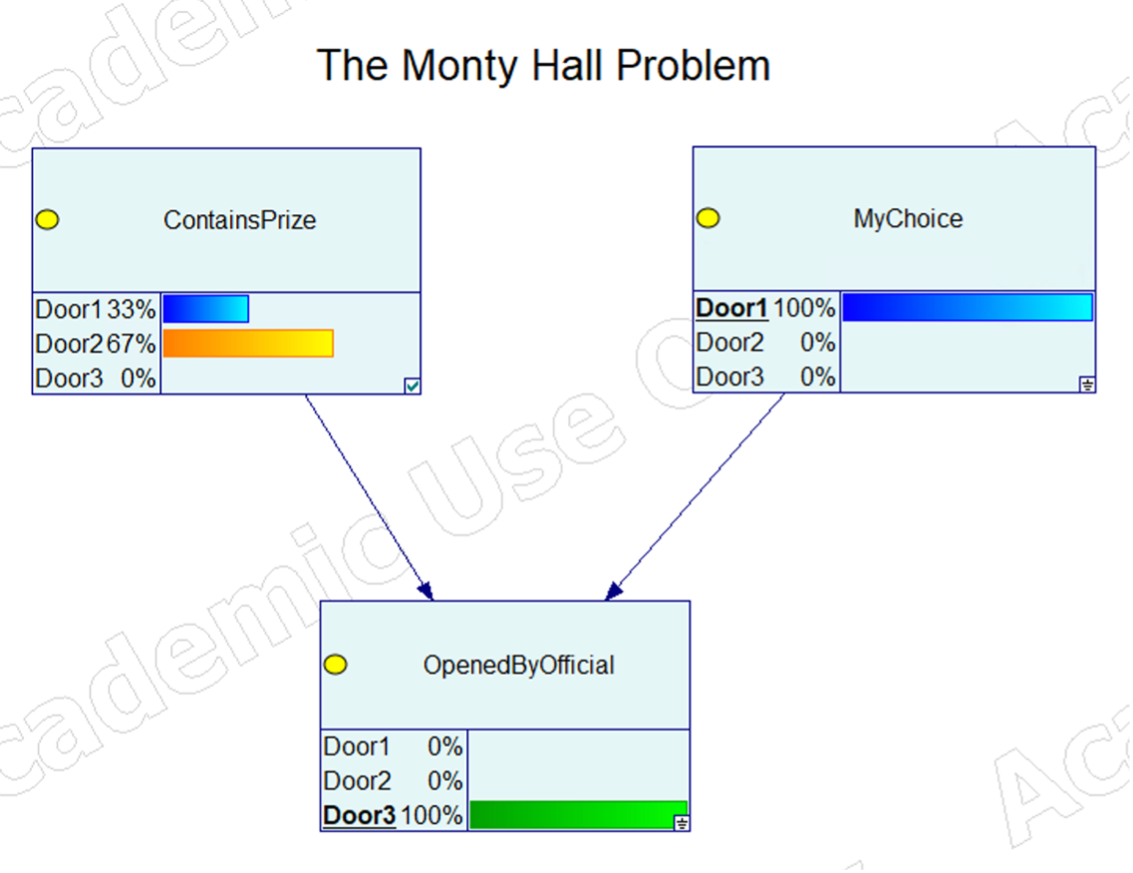
\includegraphics[width=\linewidth]{play2.png}

Result: Highest probability to win if switching door

Play 3:

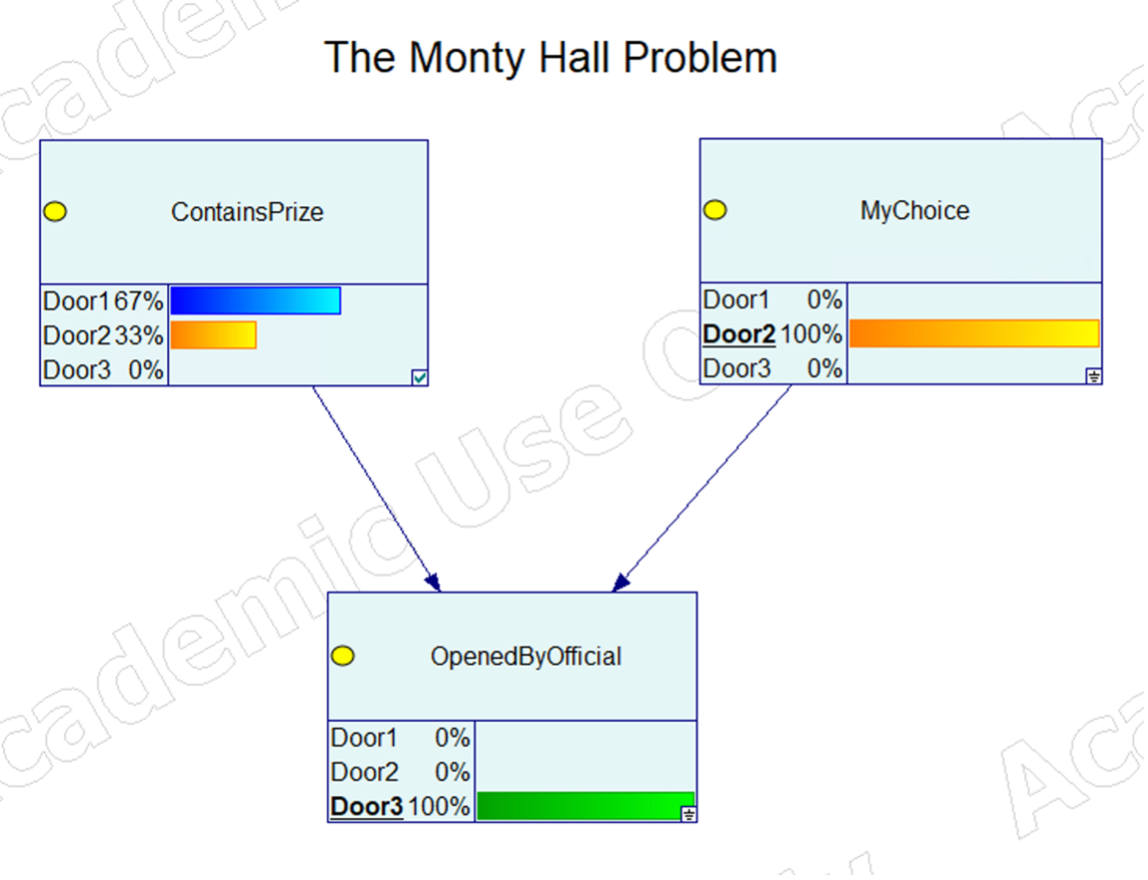
\includegraphics[width=\linewidth]{play3.png}

Result: Highest probability to win if switching door

\section*{Conclution}

From the result above, we see that the winning prize has the highest probability of being behind the door you did not choose of the two remaining after the official opened a door. It would therefore be wise to change the door when the official asks if you want to change.

\end{document}